\begin{savequote}[45mm]
\ascii{Any fool can write code that a computer can understand. Good programmers write code that humans can understand.}
\qauthor{\ascii{- Martin Flower}}
\end{savequote}

\chapter{隐式树} 
\label{ch:implicit-tree}

\begin{content}

\end{content}

\section{测试套件}

\begin{content}

如果每个用例都需要手动地执行\ascii{run},显得极其笨拙。可以将一堆测试用例打包,用一个简单的\ascii{for}循环依次执行每个用例。

\subsection{测试用例}

为了确定每个\ascii{TestCase}都被执行,可以简单定制一个计数器\ascii{num},用例执行后,断言已运行用例的数目。

\begin{leftbar}
 \begin{c++}[caption={\ttfamily{test/mars/core/TestSuiteSpec.cc}}]
#include <gtest/gtest.h>
#include "mars/core/TestCase.h"
#include "mars/core/TestSuite.h"

namespace {
  int num = 0;

  struct FooTest : TestCase {
  private:
    void runTest() override {
      num++;
    }
  };
}

TEST(TestSuite, run_multi_test_cases_using_test_suite) {
  TestSuite suite;
  suite.add(new FooTest);
  suite.add(new FooTest);

  suite.run();

  ASSERT_EQ(2, num);
}
 \end{c++}
\end{leftbar}

\subsection{通过编译}

为了快速通过编译,创建\ascii{TestSuite}的头文件。

\begin{leftbar}
 \begin{c++}[caption={\ttfamily{include/mars/core/TestSuite.h}}]
#include <vector>

struct TestCase;

struct TestSuite {
  void add(TestCase* test);
  void run();

private:
  std::vector<TestCase*> tests;
};
 \end{c++}
\end{leftbar}

\subsection{通过测试}

为了通过测试,可以快速实现\ascii{TestSuite::run}的逻辑。

\begin{leftbar}
 \begin{c++}[caption={\ttfamily{src/mars/core/TestSuite.cc}}]
#include "mars/core/TestSuite.h"
#include "mars/core/TestCase.h"

void TestSuite::add(TestCase* test) {
  tests.push_back(test);
}

void TestSuite::run() {
  for (auto test : tests) {
    test->run();
  }
}
 \end{c++}
\end{leftbar}

\subsection{内存泄露}

\ascii{TestSuite}持有若干\ascii{TestCase}实例,引入析构函数释放动态创建并添加至\ascii{TestSuite}的所有\ascii{TestCase}实例。

\begin{leftbar}
 \begin{c++}[caption={\ttfamily{include/mars/core/TestSuite.h}}]
#include <vector>

struct TestCase;

struct TestSuite {
  ~TestSuite();

  void add(TestCase* test);
  void run();

private:
  std::vector<TestCase*> tests;
};
 \end{c++}
\end{leftbar}

实现析构函数,释放动态内存。

\begin{leftbar}
 \begin{c++}[caption={\ttfamily{src/mars/core/TestSuite.cc}}]
#include "mars/core/TestSuite.h"
#include "mars/core/TestCase.h"

void TestSuite::add(TestCase* test) {
  tests.push_back(test);
}

TestSuite::~TestSuite() {
  for (auto test : tests) {
    delete test;
  }
}

void TestSuite::run() {
  for (auto test : tests) {
    test->run();
  }
}
 \end{c++}
\end{leftbar}

\subsection{消除重复}

为了消除析构函数与\ascii{run}之间的重复代码,提取一个公共的\ascii{foreach}函数。注意,不要在头文件直接实现该模板函数,最小化编译时的依赖。

\begin{leftbar}
 \begin{c++}[caption={\ttfamily{include/mars/core/TestSuite.h}}]
#include <vector>

struct TestCase;

struct TestSuite {
  ~TestSuite();

  void add(TestCase* test);
  void run();

private:
  template <typename F>
  void foreach(F f) const;

private:
  std::vector<TestCase*> tests;
};
 \end{c++}
\end{leftbar}

因此,设计得到两个独立变化的方向。

\begin{enum}
  \eitem{\ascii{迭代算法:因存储结构变化而变化(目前实现为线性列表,不排除将来实现为map);}}
  \eitem{\ascii{处理算子:存在删除,计数,运行等操作。}}
\end{enum}

可以使用\ascii{Lambda}表达式定制各种算子,实现差异化配置,实现对迭代算法的高度复用。

\begin{leftbar}
 \begin{c++}[caption={\ttfamily{src/mars/core/TestSuite.cc}}]
#include "mars/core/TestSuite.h"
#include "mars/core/TestCase.h"

void TestSuite::add(TestCase* test) {
  tests.push_back(test);
}

template <typename F>
inline void TestSuite::foreach(F f) const {
  for (auto test : tests) {
    f(test);
  }
}

TestSuite::~TestSuite() {
  foreach([](auto test) {
    delete test;
  });
}

void TestSuite::run() {
  foreach([](auto test) {
    test->run();
  });
}
 \end{c++}
\end{leftbar}

\section{嵌套结构}

为了实现更好的可扩展性,\ascii{TestSuite}不仅能打包\ascii{TestCase}实例,也应该能够打包更小的\ascii{TestSuite}的子实例,实现隐式的树结构。


\begin{figure}[H]
\centering
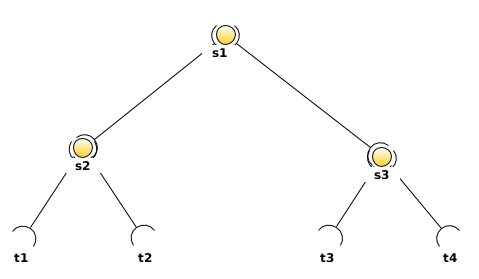
\includegraphics[width=0.8\textwidth]{figures/xunit/test-tree-example.png}
\caption{用例树:TestSuite(s1, s2, s3),TestCase(t1,t2,t3,t4)}
 \label{fig:test-case-tree}
\end{figure}

\subsection{测试依赖}

为了能够添加更多的用例,需要对计数器\ascii{num}实施初始化。当执行用例时,确保\ascii{num}被初始化为\ascii{0};否则测试用例之间存在数据脏写的错误依赖。另外,此处没有直接调用\ascii{TestSuite::run},而是使用更为抽象的\ascii{Test::run},测试装置将更加稳定。

在实现\ascii{TestSuiteSpec::run}时,显式地使用域限定符\ascii{::Test},避免与\ascii{testing::Test}产生二义性而导致编译失败。

\begin{leftbar}
 \begin{c++}[caption={\ttfamily{test/mars/core/TestSuiteSpec.cc}}]
#include <gtest/gtest.h>
#include "mars/core/TestCase.h"
#include "mars/core/TestSuite.h"

namespace {
  int num = 0;

  struct FooTest : TestCase {
  private:
    void runTest() override {
      num++;
    }
  };

  struct TestSuiteSpec : testing::Test {
  private:
    void SetUp() override {
      num = 0;  // IMPORTANT: reset counter.
    }

  protected:
    void run(::Test& test) {
      test.run();
    }
  };
}

TEST_F(TestSuiteSpec, package_multi_test_cases_into_test_suite) {
  TestSuite suite;
  suite.add(new FooTest);
  suite.add(new FooTest);

  run(suite);

  ASSERT_EQ(2, num);
}

TEST_F(TestSuiteSpec, package_sub_test_suite_into_outter_test_suite) {
  auto inner = new TestSuite;
  inner->add(new FooTest);

  TestSuite outter;
  outter.add(new FooTest);
  outter.add(inner);

  run(outter);

  ASSERT_EQ(2, num);
}
 \end{c++}
\end{leftbar}

此时,第二个测试用例编译失败。

\subsection{提取抽象}

通过提取\ascii{TestCase}与\ascii{TestSuite}的共同抽象\ascii{Test},从而使得用例的组织更加灵活。

\begin{leftbar}
 \begin{c++}[caption={\ttfamily{include/mars/core/Test.h}}]
struct Test {
  virtual ~Test() {}
  virtual void run() = 0;
};
 \end{c++}
\end{leftbar}

\subsubsection{重构TestCase}

重构\ascii{TestCase},所有显式声明的成员函数都是\ascii{private}。尤其关注被覆写的\ascii{TestCase::run},被显式地声明为\ascii{private},逼迫用户使用抽象接口\ascii{Test::run},而“面向接口编程”是一种良好的\ascii{OO}设计原则。

\begin{leftbar}
 \begin{c++}[caption={\ttfamily{include/mars/core/TestCase.h}}]
#include "mars/core/Test.h"

struct TestCase : Test {
private:
  void run() override;

private:
  virtual void setUp() {}
  virtual void runTest() {}
  virtual void tearDown() {}
};
 \end{c++}
\end{leftbar}

\subsubsection{重构TestSuite}

同理,\ascii{TestSuite}也应该被重构使用\ascii{Test}的抽象类型,而非使用\ascii{TestCase}的具体类型。

\begin{leftbar}
 \begin{c++}[caption={\ttfamily{include/mars/core/TestSuite.h}}]
#include <vector>
#include "mars/core/Test.h"

struct TestSuite : Test {
  ~TestSuite();
  void add(Test* test);

private:
  void run() override;

private:
  template <typename F>
  void foreach(F f) const;

private:
  std::vector<Test*> tests;
};
 \end{c++}
\end{leftbar}

同理,\ascii{TestSuite}的实现也应该使用\ascii{Test}的抽象类型。幸运的是,原来使用\ascii{auto}的自动类型推演,实现文件仅需要修改\ascii{TestSuite::add}函数签名便可以通过测试了。

\begin{leftbar}
 \begin{c++}[caption={\ttfamily{src/mars/core/TestSuite.cc}}]
#include "mars/core/TestSuite.h"

void TestSuite::add(Test* test) {
  tests.push_back(test);
}

template <typename F>
inline void TestSuite::foreach(F f) const {
  for (auto test : tests) {
    f(test);
  }
}

TestSuite::~TestSuite() {
  foreach([](auto test) {
    delete test;
  });
}

void TestSuite::run() {
  foreach([](auto test) {
    test->run();
  });
}
 \end{c++}
\end{leftbar}

通过\ascii{Test, TestCase, TestSuite}拼装组合,可以方便地构建复杂树形结构的用例图。

\begin{figure}[H]
\centering
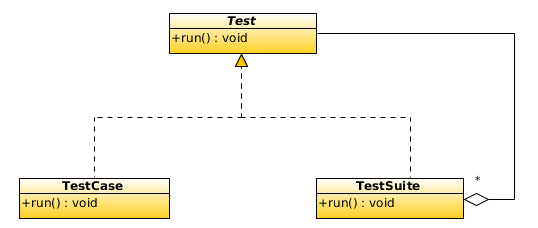
\includegraphics[width=0.8\textwidth]{figures/xunit/test-tree.png}
\caption{组合:构建隐式树}
 \label{fig:test-tree}
\end{figure}

\section{命名用例}

可以给每个\ascii{TestCase, TestSuite}命名,方便后期用例的定位与调试。

\subsection{测试用例}

\begin{leftbar}
 \begin{c++}[caption={\ttfamily{test/mars/core/TestCaseSpec.cc}}]
#include <gtest/gtest.h>
#include "mars/core/TestCase.h"

namespace {
  void assertName(const Test& test, const char* expected) {
    ASSERT_EQ(std::string(expected), test.getName());
  }
}

TEST(NamedTestCase, named_test_case) {
  assertName(TestCase("test case1"), "test case1");
}
 \end{c++}
\end{leftbar}

\subsection{通过测试}

首先,增加抽象接口\ascii{Test::getName}。

\begin{leftbar}
 \begin{c++}[caption={\ttfamily{include/mars/core/Test.h}}]
#include <string>

struct Test {
  virtual ~Test() {}
  virtual const std::string& getName() const = 0;
  virtual void run() = 0;
};
 \end{c++}
\end{leftbar}

在\ascii{TestCase}中覆写\ascii{getName}成员函数。其中,为默认构造函数提供空字符串,保证既有的用例都能通过。

\begin{leftbar}
 \begin{c++}[caption={\ttfamily{include/mars/core/TestCase.h}}]
#include "mars/core/Test.h"

struct TestCase : Test {
  explicit TestCase(const std::string& = "");

private:
  const std::string& getName() const override;
  void run() override;

private:
  virtual void setUp() {}
  virtual void runTest() {}
  virtual void tearDown() {}

private:
  std::string name;
};
 \end{c++}
\end{leftbar}

在\ascii{TestCase.cc}中实现,也极为简单。

\begin{leftbar}
 \begin{c++}[caption={\ttfamily{include/mars/core/TestCase.h}}]
#include "mars/core/TestCase.h"

TestCase::TestCase(const std::string& name) : name(name) {
}

const std::string& TestCase::getName() const {
  return name;
}

// ...
 \end{c++}
\end{leftbar}

依葫芦画瓢,\ascii{TestSuite}的名字实现与\ascii{TestCase}雷同。

\begin{leftbar}
 \begin{c++}[caption={\ttfamily{include/mars/core/TestSuite.h}}]
#include <vector>
#include "mars/core/Test.h"

struct TestSuite : Test {
  explicit TestSuite(const std::string& = "");
  ~TestSuite();

  void add(Test* test);

private:
  const std::string& getName() const override;
  void run() override;

private:
  template <typename F>
  void foreach(F f) const;

private:
  std::string name;
  std::vector<Test*> tests;
};
 \end{c++}
\end{leftbar}

\begin{leftbar}
 \begin{c++}[caption={\ttfamily{include/mars/core/TestSuite.h}}]
#include "mars/core/TestSuite.h"

TestSuite::TestSuite(const std::string& name) : name(name) {
}

const std::string& TestSuite::getName() const {
  return name;
}

// ...
 \end{c++}
\end{leftbar}

至此,测试通过。

\subsection{消除重复}

但是,\ascii{TestCase}与\ascii{TestSuite}存在结构性重复设计,包括相同的构造函数,覆写\ascii{getName}成员函数,私有字段\ascii{name}。为了消除重复,重构将公共实现搬迁至父类。

搬迁至父类需要关注两点:

\begin{enum}
  \eitem{\ascii{Test}的构造函数被声明为\ascii{public},方便子类使用\ascii{using}语句直接复用构造函数。}
  \eitem{\ascii{getName}没有必要声明为虚函数,因为在\ascii{Test}内已经完全具备实现的条件;子类强制继承\ascii{getName}的实现,拒绝被覆写。}
\end{enum}

\begin{leftbar}
 \begin{c++}[caption={\ttfamily{include/mars/core/Test.h}}]
#include <string>

struct Test {
  explicit Test(const std::string& name = "");
  const std::string& getName() const;

  virtual ~Test() {}
  virtual void run() = 0;

private:
  std::string name;
};
 \end{c++}
\end{leftbar}

\ascii{Test::getName}实现异常简单。

\begin{leftbar}
 \begin{c++}[caption={\ttfamily{src/mars/core/Test.cc}}]
#include "mars/core/Test.h"

Test::Test(const std::string& name) : name(name) {
}

const std::string& Test::getName() const {
  return name;
}
 \end{c++}
\end{leftbar}

在\ascii{TestCase}中,直接使用\ascii{using}语句复用构造函数,删除既有的\ascii{TestCase::getName}实现,及其私有字段\ascii{std::string name}。

\begin{leftbar}
 \begin{c++}[caption={\ttfamily{include/mars/core/TestCase.h}}]
#include "mars/core/Test.h"

struct TestCase : Test {
  using Test::Test;

private:
  void run() override;

private:
  virtual void setUp() {}
  virtual void runTest() {}
  virtual void tearDown() {}
};
 \end{c++}
\end{leftbar}

同理,\ascii{TestSuite}中通过相同的手段实现代码复用。

\begin{leftbar}
 \begin{c++}[caption={\ttfamily{include/mars/core/TestSuite.h}}]
#include <vector>
#include "mars/core/Test.h"

struct TestSuite : Test {
  using Test::Test;

  ~TestSuite();subsection

  void add(Testsubsection

private:
  void run() override;

private:
  template <typename F>
  void foreach(F f) const;

private:
  std::vector<Test*> tests;
};
 \end{c++}
\end{leftbar}

遗憾的是,\ascii{Test}构造函数未能声明为\ascii{protected}。但是,即使\ascii{Test}的构造函数虽然被声明为\ascii{public},设计并未丢失编译时的安全检查。因为\ascii{Test::run}被声明为纯虚函数,在编译时保证用户无法直接创建\ascii{Test}实例。

\end{content}

